\chapter{ABcast}\label{ch:abcast}

% **************************** Define Graphics Path **************************
    \graphicspath{{Chapter4-ABcast/Figs/Vector/}{Chapter4-ABcast/Figs/}}

In this chapter we  introduce a hybrid \emph{abcast} protocol, called \textsf{ABcast}, which provides non-blocking message delivery in the presence of node failures and low-latency message delivery in their absence.  This protocol was designed for use amongst $N_s1 \ldots N_sn$ nodes within the \textsf{AmaaS} system model.  

The remainder of this chapter is structured as follows:  First we introduce the rationale behind utilising a Hybrid protocol and our design approach for \textsf{ABcast}, before detailing the protocol's requirements and assumptions.  This is followed by an in-depth look at the components required by \textsf{ABcast}, and how they have been implemented.  We then explore the two protocols used to create the hybrid solution in detail, outlining each protocol's delivery and rejection criteria for \emph{abcast} messages. Finally we describe a new flow-control protocol, AFC, which has been designed specifically for use with \textsf{ABcast}.  

\section{Rationale}
    In the previous chapter we introduce \textsf{AmaaS}, a model that aims to increase the transactional throughput of distributed in-memory transactional systems.  This model depends on an \emph{abcast} protocol to maintain the replicated state between the service nodes which provide multicast ordering to client nodes; with each multicast request requiring a state change between service nodes.  For an \textsf{AmaaS} service to be viable it is vital that it provides low-latency responses to the requesting client nodes, as well as being able to handle an increasing number of client requests as the transactional system scales.  Furthermore, it is essential that such a service maintains high-availability, even in the presence of node failures, as an entire cluster of client nodes are dependent on the service.  Thus, it is essential that the underlying \emph{abcast} protocol utilised by the service can provide both non-blocking and low-latency message delivery in order to satisfy the clients requirements of highly-available and low-latency requests respectively.  
    
    \subsection{Existing Atomic Broadcast Solutions}
    The FLP impossibility \citep{Fischer:1985:IDC:3149.214121} dictates that in an asynchronous environment \emph{abcast} protocols must either admit blocking to meet its atomic guarantees or permit a likelihood of its termination guarantees not being met.  As  previously stated, known blocking protocols are of two types: GM dependent and Quorum based, both of which admit blocking in order to remain atomic.  The quorum based protocols block mildly due to false/valid suspicions of the leader node and GM protocols block severely but only in the presence of slow or crashed nodes.  
    
    Quorum based protocols provide non-blocking message delivery, however they only provide low levels of throughput as they are typically leader based, which ultimately limits the scalability of the system.  Furthermore, there is also a non-zero probability that such protocols get stuck indefinitely in a cycle of leader elections after the previous leader node is falsely suspected of crashing\footnote{This is unlikely to occur in practice with adaptive or sufficiently long timeouts used for crash-suspicion.}.  On the contrary, leaderless GM based protocols typically allow for increased levels of throughput, however the blocking inherent in GM protocols would critically undermine an \textsf{AmaaS} service's availability in the event of a service node crash.  
    
    From the disadvantages stated above, it is clear that the aforementioned protocols are not ideal when utilised within \textsf{AmaaS}.  Therefore it is necessary for a non-blocking approach to be utilised, that allows for the possibility that guarantees G1-G4 ($\S$ \ref{ssec:atomic_broadcast}) will not always be met in order to overcome the limitations of the FLP impossibility.  Utilising probabilistic guarantees on message delivery is an established technique for increasing the scalability of network multicasting systems\citep{Kermarrec:2003:PRD:766617.766623}, which has also been applied to \emph{abcast} protocols.  
    
    Felber \emph{et al.} \citep{Felber01probabilisticatomic} propose an \emph{abcast} protocol, \textsf{PABCast}, that provides probabilistic guarantees on both message \emph{safety} and \emph{liveness}.  With some non-zero probability, it is possible for only a subset of the destination set to receive a broadcast, or for all destinations to deliver the broadcast but in an inconsistent ordering.  The aim of the  \textsf{PABCast} protocol is to provide increased scalability for atomic broadcasts across large numbers of destinations, not a small subset of nodes as required by \textsf{AmaaS}.  As such the protocol does not consider throughput a primary concern.  The protocol uses \emph{rounds} to regulate when a node can initiate a broadcast and a node cannot initiate a new broadcast until all broadcasts in the current round have been delivered locally.  Ultimately this protocol structure limits a sending node to a single broadcast, which clearly limits the protocol's throughput capabilities.  
    
    In the literature, the performance of \textsf{PABCast} is evaluated using a simulation that focuses on the scalability of the system in terms of message cost as well as the likelihood of a broadcast's \emph{safety} and \emph{liveness} being violated due to the probabilistic guarantees not being met. The performance evaluation presented in the paper does not consider the throughput or latency of the \textsf{PABCast} protocol, and the protocol is only evaluated using a simulation so it is not possible to ascertain how such a protocol will function in a live asynchronous system.  It is our view that \textsf{PABCast} is not suitable for use in the \emph{AmaaS} system model.  
    
    
    \subsection{Existing Hybrid Solution}
    Bezerra \emph{et al.}\citep{6681607} propose a hybrid \emph{amcast} protocol (Optimistic Atomic Multicast) that combines a deterministic consensus protocol (Paxos), with a probabilistic protocol in order to reduce \emph{amcast} latency.  The probabilistic protocol is utilised for faster message delivery (\emph{optimisitic}), whereas Paxos is utilised to ensure correctness (determinism).  Consequently, when the probabilistic protocol delivers messages outside of the total order, it is followed up by a second, correctly-ordered delivery, which enables applications to take retrospective action to correct the ordering mistakes of the \emph{optimistic} protocol.  Hence, this approach requires both the deterministic and probabilistic protocols to finish executing in order for an \emph{amcast} to fulfil all of its guarantees. 
    
    Informally and assuming that there exists only a single group of destinations (\emph{abcast}), Optimistic Atomic Multicast works as follows:
    \begin{description}
        \item[Optimistic Delivery] \hfill
            \begin{enumerate}
                \item[1]    A \emph{abcast} $m$, is timestamped with the sending processes, $p$, clock time and broadcast to all $m.dst$.  
                
                \item[2]    Upon receiving $m$, another process $p'$, computes a wait period specific to the sender $p$, denoted as $w(p)$.  Where $w(p)$ is a delay calculated utilising the estimated clock difference between $p'$ and $p$, combined with the largest observed network latency between $p$ and $p'$.  
                
                \item[3]    $p'$ must then wait until its local clock reads $m.ts + w(p)$ before optimistically delivering $m$ ($opt\_del(m)$).  

                \textbf{Note:} A G4 violation occurs, if $m.ts$ is received at $p'$ after $m'$ has already been $opt\_del(m')$ and $m.ts < m'.ts$.  
            \end{enumerate}
        
        \item[Deterministic Delivery] \hfill
            \begin{enumerate}
                \item[4]    After $opt\_del(m)$ has been completed, it is necessary for a Paxos instance to propose $m$ to all $d \in m.dst$ to decide upon a deterministic ordering for $m$.  
                
                \item[5]    Once a consensus has been reached by Paxos for $m$, it is necessary for $m$ to be conservatively delivered to the application in its established total order ($con\_del(m)$).    
            \end{enumerate}
            
        \item[Application Level] \hfill
            \begin{enumerate}
                \item[6]    The application processes $opt\_del(m)$ messages as if the total order is correct.  However, if $m$ is later delivered in a different total order via $con\_del(m)$, then the application knows that G4 was violated by $opt\_del(m)$ and it must take retrospective action.  
            \end{enumerate}
    \end{description}
    \noindent\makebox[\linewidth]{\rule{\textwidth}{0.4pt}}

    In the context of \emph{abcast} protocols, a key disadvantage of this approach is that the deterministic protocol must always be executed in its entirety to ensure that incorrect message orderings are eventually detected.  For a message $m$, the delay between a G4 violation occurring ($opt\_del(m)$) and the Paxos execution completing ($con\_del(m)$) could be very large, as $con\_del(m)$ cannot occur until at least $m.ts + w(p) + px$; where $px$ is the time taken for Paxos to reach a consensus for $m$.   Furthermore, as Paxos is a leader based protocol, all $m$ must be processed by the leader node for a consensus to be achieved, therefore the leader node will become a bottleneck for $con\_del(m)$ under high levels of load, hence the delay between $opt\_del(m)$ and $con\_del(m)$ could become even larger.      
    
    At the application layer, a key disadvantage of Optimistic Atomic Multicast, is that two independent delivery channels must be processed by the application at anyone time ($con\_del(m)$ and $opt\_del(m)$), with the application being responsible for both detecting and recovering from G4 violations by contrasting the output of both channels.  Hence the application has to allocate additional resources for processing messages.  
    
    \subsection{Our Approach}
    Our approach is to create a hybrid protocol that combines the leaderless GM-based protocol described in section \ref{ssec:newtop}, with a custom designed probabilistic \emph{abcast} protocol that is also leaderless.  The deterministic GM protocol is utilised in the absence of crashed/suspected nodes, however in their presence the probabilistic protocol is utilised in order to overcome the blocking inherent in GM based protocols.  We refer to the probabilistic protocol as \textsf{Aramis}, and the deterministic protocol as \textsf{Base}, which when combined creates the hybrid Atomic Broadcast protocol - \textsf{ABcast}.  
    
    It should be noted that both \textsf{Aramis} and \textsf{Base} work in parallel and additional overhead is minimal as both protocols are leaderless in nature.  That is, both protocols attempt to deliver each \emph{abcast} in parallel; when the faster one succeeds in delivering a given \emph{abcast}, the slower one's attempt on that \emph{abcast} terminates.  Consequently, a given \emph{abcast} is never delivered more than once.  Typically, \textsf{Base} succeeds when there are no crashes and \textsf{Aramis} succeeds when \textsf{Base} is blocked.  
    
    \textsf{Aramis}\citep{DBLP:journals/corr/EmersonE14,EmersonTech,DBLP:conf/cloudcom/EmersonE14} is a non-blocking \emph{abcast} protocol that guarantees uniform total order (G4 $\S$ \ref{sec:atomic_guarantees}) with a probability close to 1.  \textsf{Aramis} utilises the probabilistic synchronous model ($\S$ \ref{ssec:probabilistically_synchronous}), in conjunction with closely synchronised clocks, to calculate a probabilistic upper bound on \emph{abcast} delivery times; we refer to this upper bound as a message's delivery delay, $\Delta_m$.  
    
    \subsubsection*{\textsf{Aramis: } An Informal Description}
    Upon receiving an \emph{abcast} message, a destination node waits for the calculated delivery delay to expire before delivering the message to the application.  If a message $m$ does not reach one of its destination, say $N_si$, before $\Delta_m$, then it is possible for $N_si$ to deliver a subsequent message $m'$ if $\Delta_{m'}$ expires before $m$ is received by $N_si$.  When such a scenario occurs the \emph{abcast} guarantees G4 will not be met and therefore the broadcast cannot be considered to be atomic.  
    
    A key advantage of the \textsf{Aramis} approach is that no message acknowledgements are required for a message to be delivered, instead it depends entirely on the calculated delivery delay $\Delta_m$.  Relying solely on $\Delta_m$ ensures that faulty nodes have no effect on the delivery of a message at correct nodes and it is therefore impossible for a message's delivery to become blocked.  Furthermore, as no quorums or acknowledgements are required, it is possible for  \textsf{Aramis} to tolerate at most $(n - 1)$ destination crashes when $n$ nodes are involved in an \emph{abcast}.  
    
    The \textsf{Aramis} protocol was developed to be risk adverse, with all probabilistic calculations carried out pessimistically in order to ensure that $\Delta_m$ is rarely exceeded.  Furthermore, $\Delta_m$ always assumes the worst case scenario will happen when the protocol is executing (e.g. the originator node crashes during every broadcast) to ensure that such situations are catered for.  A consequence of this pessimism, is that the latency of a \emph{abcast} message can be very large, typically 100-1000ms.  Note that these potentially large latencies, though not desirable, do not undermine \textsf{Aramis} from offering high throughput.  
    
    \subsubsection*{\textsf{Aramis} and \textsf{Base}: An Informal Description}    
    To counteract the large delivery latencies of \textsf{Aramis} it is necessary to operate a low-latency \emph{abcast} protocol, \textsf{Base}, alongside \textsf{Aramis}.  The \textsf{Base} protocol is a GM based deterministic protocol, similar to NewTop\citep{Ezhilchelvan:1995:NFG:876885.880005}, that provides low-latency high throughput \emph{abcast}s at the expense of blocking when node failures occur.  In the context of an \textsf{AmaaS} ordering service, \textsf{Base} works as follows: A message's orginator, say $m.o = N_si$, broadcasts $m$ to every $N_sj$, which in turn broadcasts an $ack_j(m)$ to every node in the service.  Once a $s$-node has received $ack_j(m)$ from all $N_sj$, $N_sj \neq m.o$, $m$ becomes deliverable.  Note that if one $N_sj$ crashes during the \emph{abcast}ing of $m$, the delivery of $m$ will be blocked if the crashed node had not sent $ack_j(m)$ before crashing and the protocol must wait for the GM service to detect the crash so that it can unblock $m$.   
    
    In order to hone the advantages of both protocols it was necessary to create the hybrid protocol \textsf{ABcast}, where an \textsf{abcast} $m$ becomes deliverable either when $\Delta_m$ has elapsed (\textsf{Aramis}) or when $ack_j(m)$ is received from every $N_sj$ (\textsf{Base}).  This approach provides the application with the low-latency of \textsf{Base} for the majority of message deliveries, whilst ensuring that a missing acknowledgement is not waited upon for more than $\Delta_m$ time.  
    
    In the event of a node failure the \textsf{Base} protocol has to wait for the GM service to detect a crash before message delivery becomes unblocked, however messages will be delivered by \textsf{Aramis} after $\Delta_m$ expires.  Therefore, when node failures are present the \textsf{ABcast} protocol will always allow for a greater throughput of delivered messages than a traditional GM based protocol, assuming that $\Delta_m$ remains smaller than the time it takes for GM to detect a node failure and construct a new service.  In the worse case, if the GM delay is smaller than $\Delta_m$, then the \textsf{Base} protocol can simply unblock its message buffer and continue to deliver messages without the use of \textsf{Aramis}.  Finally, in normal working conditions, the \textsf{ABcast} protocol should have similar performance to a traditional GM based protocol as, in the majority of cases, \textsf{Aramis} is not used for message delivery.  

As the \textsf{ABcast} protocol utilises the probabilistic protocol \textsf{Aramis}, it is possible for a node to not receive an \emph{abcast} $m$ before $\Delta_m$, resulting in that node delivering a subsequent \emph{abcast} $m'$, via \textsf{Aramis}, ahead of $m$ in the total order.  However, as previously stated, \textsf{Aramis} is carefully designed to keep the probability of meeting G4 close to 1.  Furthermore, as \textsf{Aramis} is only used when \textsf{Base} is slow or node failures occur, the probability of an \emph{abcast} message $m$ being missed in the total order is the product of two very small probabilities; \textsf{Base} not being able to deliver $m$ and \textsf{Aramis} failing $m$.  Therefore, in reality the occurrence of a node not delivering  $m$ in the correct total order is rare.   

    \subsection{ABcast Guarantees}
    Below, we state the guarantees provided by the \textsf{ABcast} protocol.  
   
    \begin{description}
    \item [\textbf{G1}] - \emph{Validity}: If the source of $m_i$ does not crash until it \emph{abcast}s $m_i$, then all operative destinations of $m_i$ deliver $m_i$.
    
    \item [\textbf{G2}] - \emph{Uniform Agreement}: If the source of $m_i$ crashes while \emph{abcast}ing $m_i$, and if any destination delivers $m_i$, then all operative
destinations of $m_i$ must deliver $m_i$.

    \item [\textbf{G3}] - \emph{Uniform Integrity}: If $m_i$ has already been delivered by a destination $d$, then $d$ cannot deliver $m_i$ again. 
    
    \item [\textbf{G4-P}] - \emph{Probabilistic Total Order}: For any two \emph{\emph{abcast}s}, $m_i$ and $m_j$, destinations that deliver both $m_i$ and $m_j$, will deliver them in an identical order with a probability $> R$.  Typically $R$ is close to $1$ ($R \rightarrow 1$).
\end{description}

\section{Assumptions}
    This section first defines the four key assumptions made when designing the \textsf{Aramis} protocol. 

    \subsection*{Assumptions:}  
    \begin{description} 
    % ******** Is this the case? Why?
        \item [\textbf{A1 - Fault Tolerance}] \hfill \\
        At most ($n-1$) of $n$ nodes involved in a broadcast can crash. However, 2 or more nodes cannot crash within an interval of some finite duration $\Delta_m$ that is smaller than a few seconds.
        
        \item [\textbf{A2 - Synchronised Clocks}] \hfill \\
        At any moment, clocks of any two operative nodes utilising \textsf{ABcast} are synchronised within $2\epsilon$ with a probability at least as large as $(1-10^{-5})$.
        
        We meet \textbf{A2} by implementing a well known probabilistic clock synchronisation algorithm \citep{Cristian:1996:SA:227210.227231}.  The details of our implementation and the parameters used are explored in $\S$ \ref{ssec:clocksynch}.       
        
        \item [\textbf{A3 - Reliable Communication}] \hfill \\
        When an operative node broadcasts $m$ to all $m.dst$, all operative destinations $d \in m.dst$ will eventually receive $m$.  
        
        We use reliable UDP protocol to guarantee that all operative nodes receive $m$ in crash-free scenarios.  However, when a broadcasting node crashes, the use of reliable UDP alone is not enough to ensure that all of the operative destinations receive $m$.  Therefore, a reliable broadcast, \emph{rbcast}, protocol will be required.  The Reliable UDP and \emph{rbcast} protocol we use are explored in detail in $\S$ \ref{ssec:reliable_udp} and $\S$ \ref{ssec:rbcast}, respectively.  
        
        \item [\textbf{A4 - Probabilistically Synchronous}] \hfill \\
        Let $x_{mx}$ be the maximum delay estimated at time $t$ by observing $NT_P$ transmissions in the recent past: The delay $x_{mx}$ will not be exceeded in any of $NT_F$, $NT_F \leq NT_P$, transmissions to unfold after $t$ with probability $(1 - q)$; where $q$ can be estimated with reasonable accuracy.  The measurement of $x_{mx}$ and $q$ are presented in section \ref{ssec:dmc}.  
        
        \textbf{A4} is motivated by previous research conducted by Ezhilchelvan \emph{et al.} \citep{Ezhilchelvan:2010:LPR:1773912.1773927} into PSM, which proposes that the challenges of designing asynchronous distributed systems, namely the FLP impossibility, can be avoided by assuming that the underlying network communication is synchronous to a given probability.  This assumption is crucial to \textsf{Aramis}'s efforts in minimising the probability of G4-P not being met.  Informally, the larger the estimated $q$, the more intensive the efforts made by \textsf{Aramis} to preserve these guarantees and \emph{vice versa}.   
        
        A consequence of A4, is that \textsf{Aramis} is not suitable for use over the Internet, or similar networks that are susceptible to large fluctuations in network delays over a short period of time.  This is because frequent occurrences of such fluctuations in $NT_F$ can lead to $q$ being underestimated, \emph{i.e.} more violations of $x_{mx}$ occur than indicated by $q$.          
    \end{description}
    
\section{ABcast Components}
In this section we detail the individual components required by the \textsf{ABcast} protocol.  For each component, we explain its purpose and design; with important implementation details highlighted where appropriate.  All of the protocols presented in this thesis are implemented in Java using the JGroups framework.  

    \begin{figure}[!h] 
        \centering    
         \includegraphics[width=0.8\textwidth]{components_no_fcc}
         \caption[\textsf{ABcast} Protocol Components Overview]{\textsf{ABcast} Protocol Components}
         \label{fig:abcast_components}
    \end{figure}
    
   Figure \ref{fig:abcast_components} provides an overview of all of the components required by the \textsf{ABcast} protocol; where GM is the Group Membership service provided by JGroups, DMC is the Delay Measurement Component (\ref{ssec:dmc}) and \emph{rbcast} is the Reliable broadcast Component (\ref{ssec:rbcast}).  

    \subsection{Clock Synchronisation}\label{ssec:clocksynch}
    In order to provide synchronised clocks between nodes executing \textsf{ABcast}, we implemented the probabilistic clock synchronisation algorithm presented in \citep{Cristian:1996:SA:227210.227231} as a dedicated protocol in JGroups.  Cristian's algorithm is a master/slave protocol, that utilises a single master node's clock time to synchronise all of the slave nodes; with each slave periodically issuing a clock synchronisation request to the master in order to synchronise their clock.  
            
            At any moment a slave's clock value is synchronised with the master node with a maximum error rate of $\epsilon$, with probability $\mathcal{P}_\epsilon \geq (1- 10^{-5})$. All of the experiments presented in this thesis utilise clock synchronisation with $\epsilon$ estimated as $1$ millisecond (ms).  A major consideration when estimating $\epsilon$ is the worst-case rate of clock drift between successive synchronisations. Ultimately, the longer the synchronisation interval, the larger the drift rate between clocks.  Estimation of $\epsilon = 1$ usually assumes an interval of $45$ minutes between synchronisations, however we use a shorter $15$ minute interval in order to increase $\mathcal{P}_\epsilon$.
            
            As each slave node synchronises its clock value with that of the master, it is possible for any two slave nodes to have a maximum error rate of $2\epsilon$.  This is because a slave $N_i$ could synchronise its clock behind the master's clock value by $\epsilon$ time.  Whereas, another slave $N_j$ could synchronise its clock ahead of the master by $\epsilon$. Hence, it is possible that $N_j.clockValue - N_i.clockValue = 2\epsilon$.  

    \subsection{Group Membership}\label{ssec:jgroups_gm}
    JGroups provides a GM service, called GMS which simply stands for Group Membership Service. GMS works as follows: upon discovering that a new node has joined the group or a node failure has occurred, GMS issues a new view to all of the protocols in the JGroups stack.  It is then the responsibility of the individual protocols to take the appropriate action when a new view is issued.  For example, unblocking message delivery if the local node was waiting for an acknowledgement from a node that is no longer present in the newly issued view.     
    
    \subsection{Reliable UDP}\label{ssec:reliable_udp}
    JGroups provides a reliable UDP protocol, \textsf{UNICAST3}, which guarantees that all UDP messages sent by a protocol higher in the network stack arrive at their destinations when node crashes do not occur.  This reliable UDP layer is placed below \textsf{ABcast} in the network stack to ensure that when messages are broadcast they are received by all destinations; where a broadcast consists of $m$ being unicast via \textsf{UNICAST3} to each of its intended recipients.  
    
    As well as providing reliable UDP unicasts, the \textsf{UNICAST3} protocol provides \emph{node-to-node} ordering as default for each message sent.  This ordering means that if a node $N_i$ sends two consecutive unicast messages, $m_1$ followed by $m_2$, to $N_j$, then $N_j$ will not deliver $m_2$ until it has first delivered $m_1$.  This behaviour is not always appropriate, therefore \textsf{UNICAST3} allows for messages to be sent Out-Of-Band (OOB), which simply means that messages will be sent reliably but they will be delivered at a destination as soon as they are received, regardless of the messages that have (or have not) been delivered before it.  Unless stated otherwise, our explanations assume that a unicast is sent using the default \textsf{UNICAST3} behaviour \emph{i.e.} not OOB.  
    
    \subsection{Reliable Broadcast}\label{ssec:rbcast}
    In the event of a node failure reliable UDP alone is not sufficient to ensure that assumption A3 holds.  This is because it is possible for a messages originator, $m.o$, to crash during the unicasting of $m$.  Assume that $m.dst = \{N_i, N_j, N_k\}$ and $m.o = N_i$, if $N_i$ crashes after unicasting $m$ to $N_j$ only, then $N_k$ will never receive $m$.  Similarly, if $N_i$ crashes during the unicasting of $m$ to $N_j$ it is possible that $N_i$ managed to send $m$ before crashing, in which case $m$ may eventually be received by $N_j$.  Both scenarios highlight that an additional protocol is required to ensure that all $m.dst$ receive $m$ in the event of $m.o$ crashing.  
    
    To overcome the limitations of Reliable UDP we have implemented a Reliable Broadcast protocol, called  \emph{rbcast}, that sits above the Reliable UDP layer in the network stack.  This protocol is inspired by the work of  Ezhilchelvan \emph{et al.} \citep{ezhilchelvanRel, ezhilchelvan2011near}, as it utilises redundant broadcasts in collaboration with PSM, to ensure that all destinations receive a broadcast.  Our \emph{rbcast} protocol has been designed specifically for use with PSM based protocols and consequently utilises some of the values from the DMC ($\S$ \ref{ssec:dmc}) as protocol parameters.  
    
    Below, we state the guarantees provided by the \emph{rbcast} protocol.  In stating them, we assume two primitives $rbcast(m)$ and $rb.deliver(m)$, which are described in detail later on in this section.
    
    \subsubsection*{Probabilistic Guarantees of \emph{rbcast}}
    
    \begin{description}
		    \item [\textbf{RB1}] - \emph{RB-Validity with Probabilistic Timeliness}: If the source of $m$ does not crash until it completes \emph{rbcasting} $m$, then all operative $s$-nodes eventually $rb.deliver(m)$, and do so within $D$ of  $rbcast(m)$ with a probability $> R$.  Typically $R \rightarrow 1$.
		    
		    \item [\textbf{RB2}] - \emph{Agreement with Probabilistic Timeliness}: If $m.o$ crashes during $rbcast(m)$ and if any $s$-node $rb.delivers$ $m$, then all operative $s$-nodes eventually $rb.deliver(m)$, and do so within $D$ of $rbcast(m)$ with probability $> R$. Typically $R \rightarrow 1$.
		
		    \item [\textbf{RB3}] - \emph{Uniform Integrity}: Any $s$-node $rb.delivers(m)$ at most once.  
    \end{description}
    
    RB1, RB2 and RB3 are directly used when implementing \textsf{Aramis}, to provide G1-G3 and G4-P, as detailed in section \ref{ssec:aramis}.  The remainder of this section describes the basic \emph{rbcast} protocol, whilst the calculations of $D$ are presented in $\S$ \ref{ssec:dmc}.
    
    \subsubsection*{The \emph{rbcast} protocol}
    All messages broadcast via \emph{rbcast} include a tuple $\{m.o, m.seq\#, m.ts\}$ that uniquely identifies the broadcast.  Where $m.o$, short for message originator, is the address of the node that initiates a broadcast message; $m.seq\#$ is a sequence number unique to each $m.o$ that is incremented after each broadcast and $m.ts$ is a timestamp of $m.o$'s synchronised clock.  Note that the first two values of the tuple are sufficient to uniquely identify a broadcast.
    
    The \emph{rbcast} protocol supports two primitives: $rbcast(m)$ and $rb.deliver(m)$.  The protocol uses a set of parameters provided by the DMC, these are:
    
    \begin{description}[leftmargin=1cm, labelindent=1cm]
        \item[$\bm{x_{mx}}$ \textnormal{and}  $\bm{q}$ - ]    As described in our assumptions.
        
        \item[$\bm{\eta}$ - ]    The delay observed between redundant broadcasts of $m$, to ensure successive broadcasts remain independent as they are passed down the network stack.  \footnote{Utilising $\eta$ ensures that lower protocols in the network stack do not bundle $m.copy = 0$ and $m.copy = 1$ into a single network packet, as this bundling would undermine the broadcasting of redundant message copies.}

        \item[$\bm{\rho}$ - ]    The number of redundant wait periods to be included into $D$ for a given $m$; the larger the value of $\rho$, the closer $R$ is to $1$.  
        
        \item[$\bm{\omega}$ - ]    A node's estimate of the networks Packet Delay Variation (PDV).  
        \end{description}
    
    \subsubsection*{$\bm{rbcast(m)}$}
    \begin{quotation}
    \noindent The primitive $rbcast(m)$ works as follows:
    \begin{enumerate}[label=\roman*]
        \item    The message to be broadcast, $m$, is created with the parameters defined above added as fields \emph{e.g.} $m.\rho, m.\eta, \ldots$ 
        
        \item    The $m$ to be $rbcast(m)$ is then broadcast two times by the originator, with the second transmission occurring $\eta$ time after the first one.  
        
        \begin{itemize}
            \item    Redundant transmissions of $m$ are distinguished by the field $m.copy$, where $m.copy = 0 \lor 1$.  
        \end{itemize}
    \end{enumerate}
        \end{quotation}

    
     \subsubsection*{$\bm{rb.deliver(m)}$}
	     \begin{quotation}
	     As soon as a copy of $m$ is received by a node, it is delivered up the stack to the higher level protocol (\textsf{ABcast}); the later copy of $m$ is not delivered up the network stack, but is used as per the \emph{rbcast} protocol.  
	     \end{quotation}
	         
     A $rbcast(m)$ is considered a success if every operative $d \in m.dst$ performs $rb.deliver(m)$.  Figure \ref{fig:rbcast} shows the \emph{rbcast} primitives and their relationship with the DMC and the underlying reliable UDP layer.  
    
    \begin{figure}[!h] 
        \centering    
         \includegraphics[width=1\textwidth]{rbcast}
         \caption[Reliable Broadcast Interactions]{Reliable Broadcast Interactions}
         \label{fig:rbcast}
    \end{figure}
    
    After $rb.deliver(m)$ has been executed, any destination $N_j$ that receives $m.copy = 0 \lor 1$ cooperates to ensure $m$ is successfully delivered by all non-crashed nodes.  Upon receiving $m.copy = 0$, $N_j$ waits to receive $m.copy = 1$ for ${t_1}$ time; where $\eta$ and $\omega$ are included in $m$'s metadata by $m.o$ ($N_i$) and ${t_1 = \eta + \omega}$.  If $t_1$ expires before receiving a subsequent copy of $m$, $N_j$ assumes that $N_i$ has crashed and starts broadcasting the largest value of $m.copy$ it has received, until $m.copy = 1$ has been broadcast. Note, $N_j$ rebroadcasts the largest copy of $m$ that it has received, as it does not know if all other $d \in m.dst$ have also received this copy of $m$.  
    
    To reduce the probability that multiple nodes are re-broadcasting $m$ simultaneously, $N_j$ waits a further $\zeta$ time to receive subsequent copy of $m$ from $m.o$, or another node in $m.dst$, before broadcasting the latest $m.copy$; where $\zeta$ is uniformly distributed on ($0,\eta$).  This process continues until all $d \in m.dst$ have received or broadcast $m$ with $m.copy = 1$.  
    
    Note that if $N_i$ does not crash, or if it crashes and an operative node receives $m$, then $m$ is broadcast \emph{at least} twice.  Conversely, if $N_i$ crashes during the initial broadcast of $m$, and no members of $m.dst - \{m.o\}$ receive a copy of $m$, then the broadcast has failed and $m$ is lost.  This is acceptable for \textsf{ABcast}, because if no $d \in m.dst - \{m.o\}$ receive $m$, then its not possible for any node to $rb.deliver(m)$, therefore it is not possible for \emph{abcast} guarantees G1 or G2 to be violated.  
    
    
    \subsubsection*{Implementation Optimisation}
    It is worth noting that in our implementations of \emph{rbcast}, every broadcast where $m.copy = 0$ is treated differently to subsequent broadcasts of $m$.  Copy 0 of $m$ is broadcast to all destinations using the default settings of Reliable UDP, i.e. messages are delivered in the same order that they were originally unicast from their source address.  This means that if node $N_i$ broadcasts $m$, followed by $m'$, it is not possible for any of the destinations to receive copy $0$ of $m'$ before it has received $m$.  This also implies that if the transmission of copy $0$ of $m$ is slow or becomes lost, than copy $0$ of $m'$ cannot be forwarded up the network stack to \emph{rbcast} protocol until $m$ has been received.  To overcome this issue all messages with $m.copy > 0$ are sent OOB to ensure that they are forwarded to the \emph{rbcast} protocol as soon as they are received at the destination node.  Therefore, if $m'.copy = 0$ has been received but not been forwarded to \emph{rbcast}, then $m'.copy = 1$ is forwarded as soon as it arrives, bypassing the backlog of messages.  
    
    The calculations used to produce $x_{mx}, \eta, \rho$ and $\omega$ are discussed in detail in $\S$ \ref{ssec:dmc}.  
    
    \subsection{Delay Measurement Component (DMC)}\label{ssec:dmc}
        For the sake of clarity, assumption A4 is repeated below:   
        
        \begin{quotation}
            Let $x_{mx}$ be the maximum delay estimated at time $t$ by observing $NT_P$ transmissions in the recent past: The delay $x_{mx}$ will not be exceeded in any of $NT_F$, $NT_F \leq NT_P$, transmissions to unfold after $t$ with probability $(1 - q)$; where $q$ can be estimated with reasonable accuracy.  
        \end{quotation}
    
        The delay measurement component is responsible for monitoring and observing the network latency of $NT_P$ transmissions from the recent past.  These latencies are then used to calculate various parameters that are required by \emph{rbcast} (and by \textsf{Aramis}) for executing \emph{abcasts} in the near future.  Being conservative, we use $NT_F = 10\%$ of $NT_P$ and $NT_P=1000$; so, a \textsf{ABcast} node freshly estimates $x_{mx}$ for every 100 new delays it observes.  Each fresh estimation of $x_{mx}$ results in the recalculation of the following parameters: $\eta, \rho, q$ and $\omega$.  
        
        Latencies are measured by the DMC based upon the timestamp $m.ts$, which is included in every message $m$ that is broadcast via the \emph{rbcast} protocol.  As the clocks of all nodes executing the \textsf{ABcast} protocol are synchronised, it is possible to measure the one-way latency of each message that is received by a node.  For example, a node $N_i$ sends an \emph{rbcast} $m$ to $N_j$, upon receiving $m$, $N_j$ immediately records the latency $x$:

        \begin{equation}
             \begin{aligned}
                 x = (N_j.clockValue - m.ts) + 2\epsilon
             \end{aligned}
        \end{equation}        
        
        It is necessary to add $2\epsilon$ to each latency to ensure that if $N_j.clockValue$ is behind $N_i.clockValue$ by the maximum error of $2\epsilon$, a positive latency value is still recorded.  
                                
        The remainder of this section explores each of the parameters provided by the DMC, explaining what they represent and how they are calculated, before providing a proof for \emph{rbcast} guarantees RB1 and RB2.  
        
        \begin{description}
        \item[\Huge$\boldsymbol{x_{mx}}$] \hfill \\
        $x_{mx}$ is simply the largest latency out of the $NT_P$ latencies observed in the recent past.  

        \item[\Huge$\boldsymbol{q}$] \hfill \\
                The parameter $q$ is the estimated probability that a transmission delay observed in the near future will exceed $x_{mx}$.  We estimate $q$ by assuming that each $x$ in $NT_p$ increases by $5\%$ in the near future.  So, the estimated set of transmission delays that exceed $x_{mx}$ in the near future is:
                
        \begin{equation}
            \begin{aligned}
                \left\{ x \text{ in } NT_p \quad  | \quad 1.05 \times x \quad > \quad x_{mx} \right\}
            \end{aligned}
        \end{equation}
                
        Note that:
         \begin{equation}
            \begin{aligned}
                1.05 \times x \quad > \quad x_{mx} \quad \Rightarrow \quad \frac{x_{mx}}{1 + 0.05 } \approx 0.95 x_{mx}
            \end{aligned}
        \end{equation}
                
        So,
            \begin{equation}
            \begin{aligned}
                q  = \frac{\text{Number of Transmissions in } NT_p \text{ that exceeds } 95\% x_{mx}}{|NT_P|}
            \end{aligned}
        \end{equation}
        
                It is possible that $q$ is calculated close to $1$ if many latencies in the recent past are within $95\%$ of $x_{mx}$.  As $q \rightarrow 1, \rho \rightarrow \infty$ so that $R$ is close to $1$.  To deal with such extreme cases, we fix an upper bound $\rho_{mx}$, $\rho_{mx} > \rho_{mn}$.  Therefore we find $q$ to be the largest value that satisfies:
                
       \begin{equation}
            \begin{aligned}
                q \quad < \quad \left(1 - \tilde{R}\right)^{\left(\frac{1}{\rho_{mx} + 1} \right)} \text{, where } \tilde{R} = R^{\frac{1}{n-1}}
            \end{aligned}
        \end{equation}

        \item[\Huge$\boldsymbol{\eta}$] \hfill \\
        $\eta$ is the parameter used by \emph{rbcast} to determine the amount of time to wait between each broadcast of a message copy and is calculated as the maximum of $x_{mx}$ and the largest delay incurred with probability $R$, when a given copy of $m$ is sent to $(n-1)$ destinations by reliable UDP.  The latter is calculated by assuming that delays are exponentially distributed with mean $\bar{x}$.  Thus,
        
        \begin{equation}
        \label{eq:eta_with_xmax}
            \begin{aligned}
                \eta = maximum \left\{ x_{mx}, -\bar{x}[\ln(1-\tilde{R})] \right\}
            \end{aligned}
        \end{equation}        
       
       where $\tilde{R} = R^{\frac{1}{n-1}}$ and $\bar{x}$ is the $67th$ percentile of delays observed in $NT_p$.  
        
        The second term in Equation \ref{eq:eta_with_xmax} turns out to be $5.3\bar{x}$ when $R = 0.99$ and $n=3$.  In general, as $R \rightarrow 1$ (\emph{e.g.} $R = 99.99\%$), $\tilde{R} \rightarrow 1$ and $\ln(1-\tilde{R}) \rightarrow -\infty$.  Therefore one may wish to define $\eta$ simply as:
        
        \begin{equation}
        \label{eq:eta_no_xmax}
            \begin{aligned}
                \eta=-\bar{x}[\ln(1-\tilde{R})]  
            \end{aligned}
        \end{equation}
        
        Equation \ref{eq:eta_no_xmax} leads to $\eta$ being immune to large outliers in $NT_p$ which exceed $-\bar{x} \times \ln(1 - \tilde{R})$ and thus inflate $x_{mx}$.  It may be unnecessary to delay the second, redundant transmission so excessively, solely in response to such large outliers.  

        \item[\Huge$\boldsymbol{\rho}$] \hfill \\
        $\rho$ is a parameter that defines the number of redundant wait periods incorporated into the calculation of $D$ so that RB1 and RB2 are met with a probability $> R$; where $R$ is a configuration parameter specified before runtime.  
        
        The probability that a given operative destination receives at least one of $m.copy = 0 \lor 1$, before $m.ts + x_{mx}$ is:
        
        \begin{equation}
            \begin{aligned}
                1 - q^{\left( 2 \right)}
            \end{aligned}
        \end{equation}
        
        Given that there can be $(n - 1)$ operative destinations at any time, we require:
        
        \begin{equation}
            \begin{aligned}
                \left[1 - q^{\left(2 \right)}\right]^{n - 1} \quad > \quad R
            \end{aligned}
        \end{equation}        
        
        As we cannot change $n$, it is necessary for us to introduce the variable $\rho$ which determines the number of additional $\eta$ length wait periods should be incorporated into $D$.  Therefore, the previous equation becomes:
        
         \begin{equation}
            \begin{split}
                \left[1 - q^{\left(\rho + 1 \right)}\right]^{n - 1} \quad > \quad R \\
                1 - q^{\left(\rho + 1\right)} \quad > \quad R^{\frac{1}{n-1}} = \tilde{R}
            \end{split}
        \end{equation}   
        
        Rearranging, taking in both sides and accounting for the fact that $\ln(a) < 0$ for  $0 < a < 1$, we set:
        
        \begin{equation}
            \begin{aligned}
                \left(\rho + 1\right) \quad > \quad \frac{\ln\left( 1 - \tilde{R} \right)}{\ln\left(q \right)}, \quad \forall \quad q \neq 1
            \end{aligned}
        \end{equation}

        \emph{i.e}:        
        
        \begin{equation} \label{eq:rho_ie}
            \begin{aligned}
                \rho \quad > \quad \frac{\ln\left(1 - \tilde{R}\right)}{\ln(q)} - 1, \quad \forall \quad q < 1
            \end{aligned}
        \end{equation}
               
        In theory, it is possible for $\rho = 0$ to be a valid parameter as it is possible for $(1-q) > R$.  However, as all of our calculations have been defined pessimistically, we define $\rho$ to be the smallest integer that satisfies:
        
        \begin{equation}
            \begin{aligned}
                \rho \quad > \quad maximum \left\{\rho_{min}, \quad \frac{\ln\left(1 - \tilde{R}\right)}{\ln(q)} - 1 \right\}
            \end{aligned}
        \end{equation}
        
        Where $\rho_{min} \geq 1$ is a configuration parameter specified before runtime; unless otherwise stated we utilise $\rho_{min} = 1$.  Observe that, for a given $R$, an integer $I =\rho_{min}, \rho_{min} + 1, \ldots$, satisfies: 

        \begin{equation}
            \begin{aligned}
                I \quad < \quad  \frac{ln \left(1 - \tilde{R}\right)}{ln(q)} - 1 \quad < \quad I + 1
            \end{aligned}
        \end{equation}
        
        for a wide range of $q$ values; e.g., for $R \approx 0.9999$

        \begin{equation}
            \begin{aligned}
                \frac{ln(1- \tilde{R})}{ln(q)}-1 < 1 \quad \forall \quad q < 0.01 = 1\%
            \end{aligned}
        \end{equation}

        This implies that small inaccuracies in estimating $q$ may not adversely affect $\rho$ estimates.  

        \item[\Huge$\boldsymbol{\omega}$] \hfill \\
        $\omega$ is the parameter utilised by \emph{rbcast} to approximate the PDV encountered by the network.  $\omega$ is simply calculated as:
        
        \begin{equation}
            \begin{aligned}
                \omega = \eta - \bar{x}
            \end{aligned}
        \end{equation}        
        
        Again, we assume exponential distribution and that $\bar{x}$ is the exponential mean of $NT_P$ observed delays.
        \end{description}

        \subsection*{Guarantees of \emph{rbcast}}
        Let $m$ be \emph{rbcast} by $N_i$, as per its clock time $m.ts$.  Let:
        
        \begin{enumerate}[label=\roman*]
            \item    $D_1 = \rho \eta + x_{mx}$
            \item    $D = x_{mx}  + 2\eta + \omega + D_1$
            \item    $D_m  = D  + 2\epsilon$
        \end{enumerate}
        
        Let $x$, as before, denote a delay (observed) and $X$ the (random) delay variable when $m$ is being \emph{rbcast}.  Finally, assume for now that $\epsilon = 0$.  
        
        \subsubsection*{RB1 - RB-Validity with Probabilistic Timeliness}        
        
        Figure \ref{fig:rbcast_calc} shows two multicasts by a correct $N_i$, with $n = 3$.  
        \begin{figure}[H]
                \centering    
                \centerline{\includegraphics[height=.4\textheight, trim=0.1cm .25cm .1cm .25cm, clip=true]{rbcast_calc_norm}}
                \caption[RB1 (RB-Validity) Calculations]{RB1 (RB-Validity) Calculations}
                \label{fig:rbcast_calc}
        \end{figure}    
        
        \paragraph{A Single Correct Destination Receives $m$}\hfill \\   
        To start with, let us focus on $m.copy = 0$ and a given correct destination, say $N_j$.  The probability that $N_j$ receives $m.copy = 0$ by its clock time $m.ts + x_{mx}$ is $(1 - q)$ by assumption A4.  \emph{i.e.} $\mathcal{P}(N_j\text{ receives } m.copy = 0 \text{ by } m.ts + x_{mx}) = (1 - q)$.  
        
        Assuming that $X$ is exponentially distributed with parameter $\lambda$, 
        
        \begin{equation}
            \begin{aligned}
                \mathcal{P}(N_j\text{ receives } m.copy = 0 \text{ by } m.ts + x_{mx})  = \left(1 - e^{-\lambda x_{mx}}\right)
            \end{aligned}
        \end{equation}
        
        Therefore,
        
        \begin{equation}
            \label{eq:1_minus_q}
            \begin{aligned}
                1 - e^{-\lambda x_{mx}} = 1 - q \implies e^{-\lambda x_{mx}} = q
            \end{aligned}
        \end{equation}
        
        Let us add one redundant wait period of $x_{mx}$.  By the property of exponential distribution,
        
        \begin{equation}
            \begin{split}
                \mathcal{P}(N_j\text{ receives } m.copy = 0 \text{ by } m.ts + 2x_{mx})  &= \left(1 - e^{-\lambda 2 x_{mx}} \right) \\
                &= \left(1 - \left(e^{-\lambda x_{mx}} \right)^2\right) \\
                &= 1 - q^2
            \end{split}
        \end{equation}
        
        Adding 2 redundant wait periods, leads to: 
         \begin{equation}
            \begin{aligned}
                \mathcal{P}(N_j\text{ receives } m.copy = 0 \text{ by } m.ts + 3x_{mx})  = 1 - q^3.
            \end{aligned}
        \end{equation}
        
        In general, with $\rho$, $\rho \geq 1$, redundant wait periods:
        \begin{equation}
            \begin{aligned}
                \mathcal{P}(N_j\text{ receives } m.copy = 0 \text{ by } m.ts + (\rho + 1) x_{mx})  = 1 - q^{(\rho+1)}
            \end{aligned}
        \end{equation}
        
        %\newpage
        \paragraph{All Correct Destinations Receive $m$}\hfill \\
%        The probability that $m.copy = 0$ is received by all $(n - 1)$ correct destinations is expressed below:
        \begin{equation}
            \begin{aligned}
                \mathcal{P}(\text{all } (n-1) \text{ correct destinations receive } m.copy = 0 \text{ by } \\ 
                m.ts + (\rho + 1) x_{mx})  = \left[ 1 - q^{(\rho+1)} \right] ^ {n - 1} > R
            \end{aligned}
        \end{equation}
        
        If there are fewer correct destinations then $(n -1)$, say $(n - 2)$, then the above probability is:
        \begin{equation}
            \begin{split}
                \left[ 1 - q^{(\rho+1)} \right] ^ {n - 2} > \left[ 1 - q^{(\rho+1)} \right] ^ {n - 1} > R 
            \end{split}
        \end{equation}
        
        When $\eta \geq x_{mx}$ (see Equation \ref{eq:eta_with_xmax}):
        \begin{equation}
            \begin{aligned}
                D = \eta\rho + x_{mx} \geq \rho x_{mx} + x_{mx} = (\rho + 1) x_{mx}
            \end{aligned}
        \end{equation}
        
        Moreover, $D > D_1$, so:
        \begin{equation}
        \begin{aligned}
                \mathcal{P}(\text{all } (n-1) \text{ correct destinations receive } m.copy = 0 \text{ by } \\
                 m.ts + D)  > \left[ 1 - q^{(\rho+1)} \right] ^ {n - 1} > R
            \end{aligned}
        \end{equation}
                
        Accounting for $\epsilon > 0$ and recalling $D_m = D + 2\epsilon$:
        \begin{equation}
        \begin{aligned}
                \mathcal{P}(\text{each correct destinations receives } m.copy = 0 \text{ by \underline{its} clock time } m.ts + D_m) > R
            \end{aligned}
        \end{equation}
        
        \textbf{Note:} The RB-Validity property is met when a correct $N_j$ receives either $m.copy = 0$ or $m.copy = 1$ by its cock time $m.ts + D_m$.  Since, $\rho \geq 1$,
        
         \begin{equation}
        \begin{aligned}
                \mathcal{P}(\text{RB-Validity is met within } D_m) > \\ \mathcal{P}(\text{Each correct } N_j \text{ receives } m.copy = 0 \text{ by its clock time } m.ts+D_m) \\ > R
            \end{aligned}
        \end{equation}
        
        
    \subsubsection*{RB2 - Agreement with Probabilistic Timeliness}
    Suppose now that $N_i$ crashes before completing the redundant transmissions of $m$ and $n>2$.  Suppose also that only one node, $N_j$, has $m$ with $m.copy=0$. This is the worst case to be considered because if $N_j$ $m.copy>0$, then $N_i$ crashed only after it completed broadcasting $m.copy \geq 0$, therefore some node other than $N_j$ also has $m$; the more destinations which receive some copy of $m$, the more likely it is that $rbcast(m)$ is completed.  On the other hand, if no destination receives any copy of $m$ from the crashed $N_i$, then the case for discussion does not exist.  
    
    If copy $m.copy = 0$ takes at most $x_{mx}$ to reach $N_j$ (which occurs with probability ($1-q$)), $N_j$ would start disseminating on behalf of $N_i$ at or before time:
    
    \begin{equation}
    \label{eq:replace_zeta}
             \begin{aligned}
                m.ts+ x_{mx} + \eta + \omega +\zeta
             \end{aligned}
         \end{equation}    
    
    Recall that $\zeta$ is the random wait that all disseminating nodes must observe before disseminating $m$, with $\zeta$ uniformly distributed on ($0, \eta$).  Therefore, in our calculations we assume that the observed $\zeta$ is the largest value possible, $\eta$ and $\zeta$ in equation \ref{eq:replace_zeta} is replaced by $\eta$ in the discussions below.  Figure \ref{fig:rbcast_a_delay} shows the worst case scenario when $n=3$.  
    
    \begin{figure}[H]
                \centering    
                \centerline{\includegraphics[height=0.4\textheight, trim=0.1cm .25cm .1cm .25cm, clip=true]{rbcast_calc_agreement_delay}}
                \caption[RB2 Calculations - Worse Case]{RB2 Calculations - Worse Case}
                 \label{fig:rbcast_a_delay}
        \end{figure} 
    
    \paragraph{Simplified Scenario} \hfill \\    
    As before, we assume that propagation delays are exponentially distributed with parameter $\lambda$.  Also suppose, for now, that $\epsilon = 0$ and $N_j$ instantaneously transmits its $m.copy = 0$ without waiting for $(\eta + \omega)$ and a random wait \footnote{Both of these simplicity assumptions will be removed shortly.}.  
    
        \begin{figure}[h]
                \centering    
                \centerline{\includegraphics[height=0.4\textheight, trim=0.1cm .25cm .1cm .25cm, clip=true]{rbcast_calc_agreement_no_delay}}
                \caption[RB2 Calculations - Simplified Scenario]{RB2 Calculations - Simplified Scenario}
                \label{fig:rbcast_a_no_delay}
        \end{figure} 
        
    Of interest, is the probability, $P_{D2}$, that a given node, $N_k$ receives $m.copy = 0$ from $N_j$ by $m.ts + D_2$; where $D_2 = (\rho + 2) x_{mx}$.  Recall that $q  = e^{-\lambda x_{mx}}$ by the exponential assumption.  The time when $N_k$ receives $m.copy = 0$ is determined by the sum of two independent exponential delays (see Figure \ref{fig:rbcast_a_no_delay}):
    \begin{enumerate}[label=\roman*]
        \item    $N_i$ to $N_j$
        \item    $N_j$ to $N_k$
    \end{enumerate}
    
    This sum follows Erlang distribution with parameter $\lambda$ and number of \emph{hops}, $k$, $k = 2$.  So,
    
    \begin{equation}
        \label{eq:pd_2_original}
        \begin{split}
                P_{D2} &= 1 - \sum\limits_{n=0}^{k-1}\left[ \left(\frac{1}{n!}\right) e^{-\lambda D_2} \left( \lambda D_2 \right)^n  \right] \\
                &=    \left[ e^{-\lambda D_2} + e^{-\lambda D_2}\left( \lambda D_2 \right)     \right] \\
                &=    \left[ e^{-\lambda D_2} \left( 1 + \lambda D_2 \right)    \right]
        \end{split}
    \end{equation}
        
        Recall that $e^{-\lambda x_{mx}} = q$ (see equation \ref{eq:1_minus_q}),
        
        \begin{equation}
        \begin{split}
               -\lambda x_{mx} &= \ln(q) \\
               e^{-\lambda D_2} &= e^{\lambda (\rho + 2) x_{mx}} = q^{(\rho+2)} \\
               \lambda D_2 &= \lambda x_{mx} (\rho + 2) = - (\rho + 2) \ln(q)
        \end{split}
    \end{equation}
            
    From equation \ref{eq:pd_2_original}:
    
    \begin{equation}
        \label{eq:pd_2_second}
        \begin{split}
                P_{D2} &= 1 - \left[ q ^{(\rho + 2)} \left( 1 - (\rho + 2) \ln q \right)   \right] \\
                           &=  1 - q^{(\rho + 1)} \left[ q \left( 1 - (\rho + 2) \ln q  \right) \right] \\
                           &= 1- q^{(\rho + 1)} \left[ q - (\rho + 2) q \ln q \right]
        \end{split}
    \end{equation}
    
    % 0_+ = Max{0, x}
    Let $q \ln q = 0$.  As $q$ values are $q \rightarrow 0_+$ typically small, we approximate:
    
    \begin{equation}
        \begin{aligned}
                q - (\rho + 2) q \ln q \lesssim 1
            \end{aligned}
        \end{equation}
    
    So, applied to Equation \ref{eq:pd_2_second} we get:
    
    \begin{equation}
        \begin{aligned}
                P_{D2} = 1 - q^{(\rho+1)} \left( q - (\rho + 2) q \ln q)    \right) \gtrsim 1 - q^{(\rho + 1)}
            \end{aligned}
        \end{equation}
        
        Therefore, the probability that all $(n-2)$ correct $N_k$ receive $m.copy = 0$ from $N_j$ by $m.ts + D_2$ is:
        
    \begin{equation}
        \begin{aligned}
                \left[P_{D2} \right]^{n-2} \gtrsim \left[ 1 - q^{(\rho+1)} \right] ^{n-2} > \left[ 1 - q ^{(\rho + 1)}\right]^{n-1} > R
        \end{aligned}
    \end{equation}
    
    
    When $\eta \geq x_{mx}$,
    
    \begin{equation}
        \begin{aligned}
                D - \left( 2 \eta + \omega \right) = \rho \eta + 2 x_{mx} \geq (\rho + 2) x_{mx}
            \end{aligned}
        \end{equation}
        
    Thus, the probability that every correct $N_k$ receives $m.copy = 0$ from $N_j$, by ${m.ts + D - (2\eta + \omega)}$, is larger than ${\left[P_{D2}\right]^{(n - 2)} > R}$.  

    \paragraph{Simplifications Removed} \hfill \\    
    Accounting for the fact that $N_j$ \emph{rbcasts} $m$ within at most $(2 \eta + \omega)$ time after receiving $m.copy = 0$ from $N_i$ and $\epsilon \neq 0$:
    
    \begin{equation}
        \begin{aligned}
                \mathcal{P}(\text{each correct } N_k \text{ receives } m.copy = 0 \text{ by \underline{its} clock time } m.ts + D + 2\epsilon) > R
         \end{aligned}
    \end{equation}
    
    Thus, the agreement property is met for the delay of $D_m = D + 2\epsilon$, with probability $> R$.  
    
    \paragraph{Remarks} \hfill \\
    The simplifying approximation $(q - (\rho + 2) q \ln q)$ is not unreasonable; it evaluates to be $0.80$ and $0.95$ when $q = 5\%$ and $\rho = 3$ and $\rho = 4$, respectively.  Other than this approximation, the agreement anaylsis is pessimistic by considering the worse-case crash scenario.  When $N_i$ crashes during a multicast, several scenarios are possible, with just some or all destinations receiving $m.copy = 0$.  In the former case, several $N_j$ may multicast $m.copy = 0$, increasing the chances of the other destinations receiving $m.copy = 0$ within $D_m$.  In the latter case the analysis is similar to that presented for RB-Validity.  
    
   
\clearpage
\section{Atomic Broadcast Protocol}\label{sec:ABcast}
Hitherto this chapter has focused on the underlying assumptions made when designing the \textsf{ABcast} protocol and the components it requires to function.  This section focuses on how the hybrid protocol functions, detailing the specifics of both the \textsf{Aramis} and \textsf{Base} protocols.  First we explore the \textsf{Base} protocol, as this protocol will be responsible for the majority of message deliveries and is the more conventional of the two \emph{abcast} protocols.  We then explore the \textsf{Aramis} protocol, detailing how it utilises the guarantees of \emph{rbcast} to calculate $\Delta_m$.   This followed by a formal definition of \textsf{ABcast}'s delivery conditions.  Finally, we discuss how the \textsf{ABcast}'s reliance on the DMC requires an initialisation period to be observed by the protocol before \emph{abcast}ing can begin.  

    \subsection{Base}
    The \textsf{Base} protocol is based upon the NewTop \citep{Ezhilchelvan:1995:NFG:876885.880005} algorithm discussed in $\S$ \ref{ssec:newtop}, with a few key differences motivated by our use of synchronised clocks and PSM.  
    
    The \textsf{Base} protocol works as follows when a node $N_i$ sends an \emph{abcast} $m$: $N_i$ \emph{rbcast}s $m$, and as per the \emph{rbcast} protocol $m$ is assigned an id tuple $\{m.o, m.seq\#, m.ts\}$.  This tuple is utilised by \textsf{Base} to specify the total order of $m$, with all destinations in $m.dst$ ordering messages in ascending order based upon their timestamp.  In the event of any two messages having the same $m.ts$ value, the address specified in $m.o$ is used for tie-breaking to ensure a total order; note this is highly unlikely in practice as $m.ts$ is recorded in nanoseconds.  Similarly, in our implementation it is not possible for the same node to \emph{rbcast} two messages with the same $m.ts$, as a single thread called the \emph{sender} thread, is used for sending all $m$ with $m.copy = 0$.  
    
    Like NewTop, delivery of $m$ is blocked until each $d' \in m.dst - \{m.o\}$ has acknowledged $m$ by sending $ack_{d'}(m)$ to every $d \in m.dst$ and all $d \in m.dst$ have received $ack_{d'}(m) \forall (m.dst \setminus \{m.o,d\})$, thus C1 ($\S$ \ref{ssec:atomic_broadcast}) is met.  With each acknowledgement consisting of the id tuple that belongs to the message being acknowledged.  
    
    The use of synchronised clocks to uniquely timestamp each message, removes the need for tentative timestamps to be shared between destinations.  Instead the ordering of a message is dictated from its inception based upon its timestamp.  However,  a message's final place in the total order is not known by a destination until it has received an acknowledgement from all other $d' \in (m.dst - \{m.o\})$.  Figure \ref{fig:base_flow} shows the message flow required by the base protocol in order for an \emph{abcast} to be delivered.  
    
    \begin{figure}[!h] 
        \centering    
         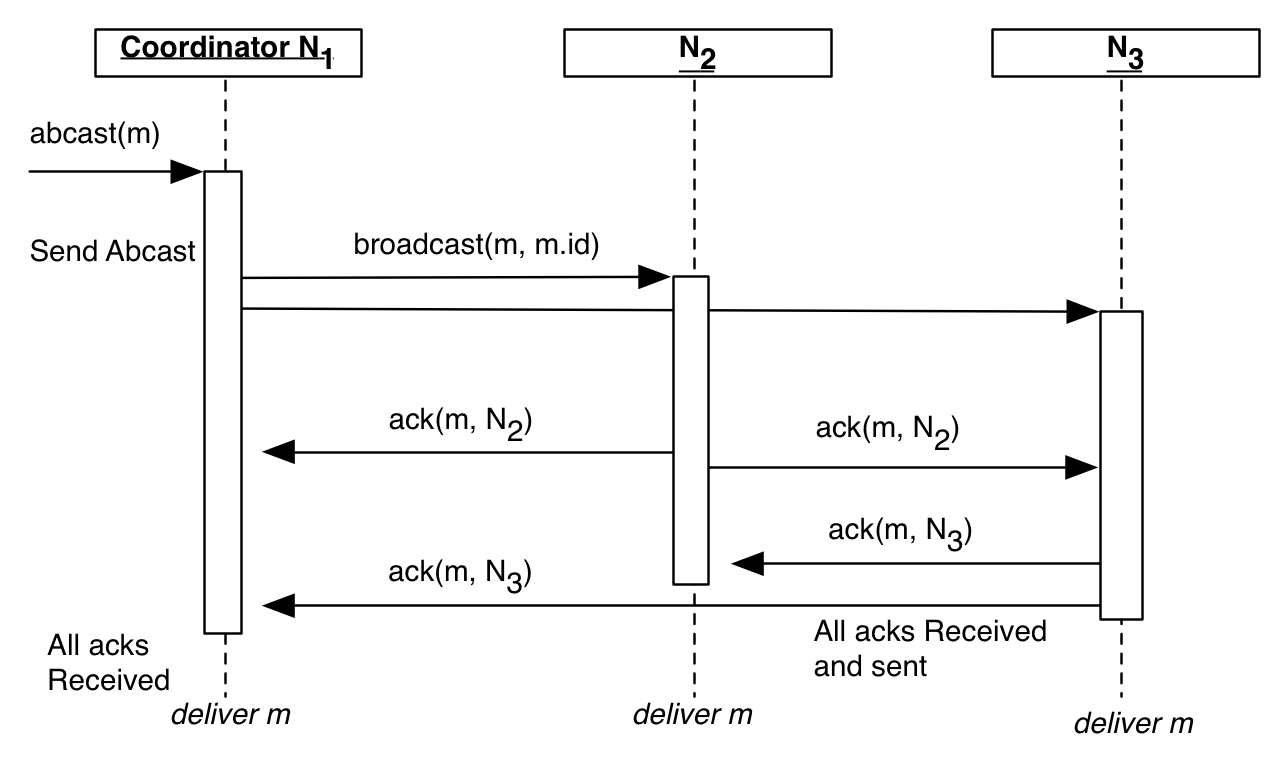
\includegraphics[width=0.85\textwidth]{Base}
         \caption[\textsf{Base} Atomic Broadcast protocol]{\textsf{Base} Atomic Broadcast protocol}
         \label{fig:base_flow}
    \end{figure}  
    
    In order to overcome C2, as described in \ref{sec:atomic_guarantees}, and ensure that G3 and G4 are respected, it is necessary for each $d \in m.dst$ to maintain a vector clock \citep{Mattern88virtualtime, fidge1988timestamps}; with each $d$'s vector clock stating the last $rbcast(m)$ sent by $d$ as well as the the latest $m$ to be $rb.delivered$, by $d$, that originated from each $d' \in (m.dst - d)$ \footnote{Where the latest $m$, is defined as the message containing the largest timestamp from a given $d'$}.  This vector clock is then included in every $m$ and $ack_{d'}(m)$ sent by a node.  
    
    For any message $m$, regardless of whether it originated at the current node, it is necessary for the associated acknowledgements and vector clocks to be checked to see if a message is missing from the total order before $m$ can be delivered.  If a node $N_i$ has not received $m$, but has learnt of its existence via a \emph{vector clock} or an acknowledgement, then we consider $m$ to be \emph{known} by $N_i$.  The \textsf{Base} delivery conditions are formalised below:
    
    \paragraph{\textsf{Base} Delivery Rule:}\hspace{0pt} \\
        A node, $N_j$ delivers any $m$, via \textsf{Base}, only after $D1_B$ and $D2$ stated below are satisfied:
        \begin{description}[labelindent=1cm]
            \item[$\boldsymbol{D1_B}$] - $m$ is acknowledged by all nodes other than $m.o$. 
            \item[$\boldsymbol{D2}$] - all \emph{known} $m'$, with $m'.ts < m.ts$ have been delivered.
        \end{description}
    
    \subsubsection*{Acknowledgement Piggybacking}\label{ssec:base_ack_piggyback}
    In the explanation of \textsf{Base} we assume that each acknowledgement is explicitly sent as dedicated message, however in practice this is an expensive operation in terms of both latency and bandwidth.  Therefore in our implementation of \textsf{Base} we piggyback message acknowledgements on subsequent \emph{rbcast}s sent by an the acknowledging node; acknowledgements are piggybacked onto all copies of $m$, i.e. all $m.copy =0, 1$, or not at all.  Of course this is only appropriate if there is a message waiting to be \emph{rbcast}, otherwise deadlock will occur at all $d \in m.dst$ as an acknowledgement will never be sent.  Consider, node $N_j$ is attempting to send $ack_{N_j}(m)$ to $N_i$, if $N_j$ does not receive an \emph{abcast} request within $\mathcal{A}_d$ time, then an explicit acknowledgement message is sent to $N_i$ containing $ack_{N_j}(m)$, as well as any other pending acknowledgements.  We define $\mathcal{A}_d$ as $\mathcal{A}_d = 2\eta + \omega$ and an explicit acknowledgement as being a dedicated message $m_{ack}$ that is unicast to all $d \in m.dst$ and is not assigned a \emph{rbcast} id; hence only a single copy of $m_{ack}$ is broadcast via reliable UDP.  \footnote{Explicit acknowledgements are not \emph{rbcast} in order to further minimise the bandwidth cost of sending $m_{ack}$.}
    
%    \subsubsection*{Aborting rho > 0}
%    Another possible optimisation is for the redundant multicasting of $rbcast(m)$, to be aborted once $m$ is known to have been acknowledged by all destinations; this includes destinations that are disseminating $m$ or waiting on $m.copy > 0$.  The logic for this optimisation is as follows: If a node $N_i$ has delivered $m$ locally, then we know that all other $d' \in m.dst$ must have received $m$ as $N_i$ must have received $ack_{d'}(m)$ from all $d' \in m.dst$ in order for $m$ to have been delivered locally.  Therefore it is safe to abandon the \emph{rbcast}ing of $m$ as all $m.dst$ have received at least one copy of $m$. 
%    
%    Note, this optimisation has \textbf{not} been utilised in our implementation of the \textsf{ABcast} protocol.  This optimisation is not possible if a message has been delivered locally by the \textsf{Aramis} protocol as it is impossible to know for certain that all $d' \in m.dst$ have received $m$.  

    \subsection{Aramis}\label{ssec:aramis}
    As previously stated,  \textsf{Aramis} is a non-blocking probabilistic \emph{abcast} protocol that utilises a calculated delivery delay $\Delta_m$ to place an upper bound on message deliveries.  The \textsf{Aramis} protocol works in conjunction with \textsf{Base} to ensure that message delivery does not become blocked in the event of slow or crashed nodes.  However, the \textsf{Aramis} protocol does not simply deliver each received message after $\Delta_m$ has expired, as this could cause a \emph{known} message to be missed in the total order.  Instead, it utilises the acknowledgements and \emph{vector clocks} that are integral to \textsf{Base} to ensure that \emph{known} messages are not missed from the total order.  Therefore, if a message $m$'s $\Delta_m$ delay expires, the message can only be delivered after all \emph{known} messages that precede $m$ in the total order have been delivered.  The \textsf{Aramis} delivery conditions are formalised below:
    
    \paragraph{\textsf{Aramis} Delivery Rule:}\hspace{0pt} \\
        A node, $N_i$ delivers any $m$, via \textsf{Aramis}, only after $D1_A$ and $D2$ stated below are satisfied:
        \begin{description}[labelindent=1cm]
            \item[$\boldsymbol{D1_A}$] - The clock of $N_i > m.ts + \Delta_{m}$, where $\Delta_{m} = 2(D + \epsilon) + \mathcal{A}_d$.
            
            \item[$\boldsymbol{D2}$] - All \emph{known} $m'$, with $m'.ts < m.ts$ have been delivered.
        \end{description}
    
    
        \subsubsection*{Calculating $\boldsymbol{\Delta_m}$}
        Let us, for simplicity, assume that $\epsilon = 0$.  The explanation is twofold.  First, recall that \emph{rbcast} guarantees on agreement: if $N_i$ \emph{rbcast}s $m$ and if any operative $s$-node (be it $N_i$ or otherwise) $rb.delivers$ $m$, all destination nodes $rb.deliver$ $m$ within $m.ts + D$ with probability $> R$.  
        
        Secondly, the aim of \textsf{Aramis} is to aid the delivery of \emph{abcast} messages when \textsf{Base} is blocked due to node crashes.  So, delivery by \textsf{Aramis} is delayed until all acknowledgements are $rb.delivered$ when there are no crashes.  Since an operative node can acknowledge at most $\mathcal{A}_d$ time after $rb.delivering$ $m$, we have:
        
        \begin{equation}
            \begin{aligned}
                \Delta_m \geq D + \mathcal{A}_d + D
            \end{aligned}
        \end{equation}
        
        Accounting for the clock synchronisation error rate of $2\epsilon$, we calculate $\Delta_m$ as:
        
        \begin{equation}
            \begin{aligned}
                \Delta_m = 2(D + \epsilon) +  \mathcal{A}_d
            \end{aligned}
        \end{equation}
        
        \textbf{Note:} By delivering $m$ at $m.ts + \Delta_m$, $\Delta_m > 2 \times D$, \textsf{Aramis} indeed meets the total order (G4-P) guarantee with a probability much larger than the user specified value of $R$. 
                
        \subsection{Aramis and Base - \textsf{ABcast}}
        The \textsf{ABcast} protocol, is a hybrid solution that combines the delivery conditions of the \textsf{Aramis} and \textsf{Base} protocols.  Here we present a concise formalisation of the delivery rule for the entire \textsf{ABcast} protocol.  A node, $N_j$ delivers any $m$ via \textsf{ABcast}, only after both $D1$ and $D2$ stated below are satisfied:
	    \begin{description}[labelindent=1cm]
	        \item[$\boldsymbol{D1}$] - The clock of $N_i > m.ts + \Delta_{m}$ ($D1_A$) or $m$ is acknowledged by all nodes other than $m.o$ ($D1_B$). 
	        
	        \item[$\boldsymbol{D2}$] - All \emph{known} $m'$, with $m'.ts < m.ts$ have been delivered.
	    \end{description}
	    
        \subsubsection*{Extremely Delayed \emph{rbcast} Messages}\label{ssec:abcast_rejection}
        As \textsf{Aramis} is a probabilistic protocol it is possible for a message $m$ to be $rb.delivered$ at destination $d$, after its proceeding message $m'$ in the total order has already been $ab.delivered$; where $ab.delivered$ refers to a $m$ being delivered by \textsf{ABcast}. In such a case, there is one of two actions possible:

         \begin{itemize}
            \item    Discard $m$ when it becomes known to $d$; resulting in a violation of G1 and G2.  
            
            \item    Deliver $m$ to the application via an exception; resulting in a violation of G4.  
        \end{itemize}                       
        
        \textsf{Aramis} takes the second option and throws an exception when a $rb.delivered$ message is not $ab.delivered$; we refer to this process as a message being \emph{rejected}.  Explicitly \emph{rejecting} a message from the $ab.delivery$ allows for higher levels in the network stack (e.g. \textsf{SCast}) to initiate an appropriate recovery mechanism to mitigate the effects of G4 ordering violations on the system's state.  Furthermore, as the \emph{rejected} message is still being delivered to the application, albeit via an exception, it is possible for the payload of the \emph{rejected} message to be utilised by the application as part of its recovery mechanism for ordering violations.    
        
        \subsubsection*{Message Rejections}
        A message, $m$, sent by node $N_i$, can only be \emph{rejected} by another recipient, $N_j$, when a message $m'$ from $N_j$ has been incorrectly delivered before $m$ in the total order; where $m.ts < m'.ts$ but $m'$ is incorrectly $ab.delivered$ first.  In order for $m'$ to be $ab.delivered$ ahead of $m$, resulting in $m$ being \emph{rejected} by $N_j$, it is necessary for both of the statements below to be true:
        
        \begin{enumerate}
            \item    $N_j$ \emph{rbcasts} $m'$ with $m'.ts > m.ts$, but $m$ is not $rb.delivered$ by $N_j$ before $m'.ts + \Delta_{m'}$.
            
            \item    $N_j$ does not receive an acknowledgement for $m$, or any \emph{rbcasts} sent after $m$ by $N_i$, before $m'.ts + \Delta_{m'}$.  
        \end{enumerate}
        
        If condition one is not true, i.e. $N_j$ $rb.delivers$ $m$ before $m'.ts + \Delta_{m'}$, then $N_j$ has received $m$ before $m'$'s delivery time and therefore $N_j$ will not miss $m$ in the total order.  Similarly, if condition two is not true, then $N_j$ will know that a message sent by $N_i$ is missing as soon as it inspects the received acknowledgement, attached \emph{vector clock} or the $seq\#$ of the $rb.delivered$ message.  When both conditions hold, it is guaranteed that $m'$ will be $ab.delivered$ via \textsf{Aramis}, as it is impossible for \textsf{Base} to $ab.deliver$ a message if condition two is true.  
        
        The rules presented above can be extended to cater for when $n > 2$.  Assuming the same scenario described above, we introduce $N_k$ which represents all nodes involved in an \emph{abcast} that are not $N_i$ or $N_j$.  A message is \emph{rejected} by a node $N_j$ if conditions $1$ and $2$ are true, as well as the condition stated below:
        
         \begin{itemize}
            \item[3.] $N_j$ does not $rb.deliver$ an acknowledgement of $m$ from any $N_k$, and it does not $rb.deliver$ a \emph{rbcast} from any $N_k$, that has $rb.delivered$ $m$, before $m'.ts + \Delta_{m'}$ \footnote{Where $m'.ts + \Delta_{m'}$ is based upon $N_j$'s local clock.}.  
        \end{itemize}
        
        If conditions $1,2$ and $3$ are true it is not possible for $m$ to be known by $N_j$ before $m'.ts + \Delta_{m'}$.  This is because $m$ has not been $rb.delivered$ by $N_j$ and $N_j$ does not know of $m$, as $m$ has not been acknowledged, or described in a vector clock, by any $N_k$, before $m'$ is $ab.delivered$ by $N_j$.  
        
        
    \subsection{Initialisation Period}
     The \textsf{ABcast} protocol requires a \textquoteleft{}warm-up' period before \emph{abcast}s can be sent between nodes.  This period is required in order to: 
    
    \begin{enumerate}[label=\roman*]
        \item    Synchronise the clocks of all participating nodes in the view.
        
        \item    Ensure that each node's DMC has recorded at least $NT_p$ latencies
    \end{enumerate}         
     
     Synchronisation must be performed first as the DMC is dependent on this assumption.  Our solution to recording $NT_p$ latencies, is to incorporate a mandatory \emph{probing} period that must be observed by all nodes in the current view after their clocks have been synchronised and before \emph{abcast}ing can begin.  

    The probing period required during initialisation utilises \textquoteleft{}empty' probe messages to record $NT_p$ latencies at each node's DMC.  An empty probe consists of a message, with a payload the size of those expected during \emph{abcast}ing, being unicast to all $n$ nodes in the current view.  This requires each node in the view to send at least $\frac{NT_P}{n}$ probes, however in reality the number should be higher to take into account that nodes will start the initialisation process at different times.  With each subsequent probe being broadcast $x$ time apart; with $x$ being a value determined before run-time that should be an approximation of the expected frequency of \emph{abcast}s.  Once all nodes in the view have sent their probes, and recorded at least $NT_p$ latencies, it is possible for this node to start executing \emph{abcast}s.  
    
    A disadvantage of utilising empty probes is the risk of network latencies being over-or underestimated respectively, due to unknown load conditions that an application would experience later.  Such inaccuracies are corrected as the application progresses and will not be an issue if crashes do not occur at the start of the application.  

        
    \subsection{Initialising a Newly Joined Node}
    When a new view is issued containing a new node, $N_i$, it is necessary for $N_i$ to undergo an initialisation period similar to that described in the previous section.  Clock synchronisation is simple, as $N_i$ can just contact the designated master node (as per \citep{Cristian:1996:SA:227210.227231}) and initiate the synchronisation protocol.  
    
    Recording the required $NT_p$ latencies is slightly trickier, as utilising a probing period similar to the initialisation period could have an adverse effect on all other nodes in the view.  This is because the existing nodes will most likely be heavily loaded from application requests, hence the need for an additional $s$-node, and adding additional load over a short period of time would be detrimental to performance.  Therefore, we propose that a better solution would be for new nodes to be \emph{silent watchers} until $NT_p$ latencies have been recorded.  A silent watcher, is a node that receives \emph{abcast}s from all other nodes in the view, but is unable to initiate its own \emph{abcast}s until after it has received $NT_p$ \emph{abcast}s and hence recorded $NT_p$ latencies.  When a new view is issued by the GM service, existing nodes include $N_i$ in the destination set of subsequent \emph{abcast}s, resulting in $N_i$ eventually receiving $NT_p$ messages.  
    
    \textbf{Note:} While $N_i$ is considered a silent watcher, it is still possible for it to participate in the redundant \emph{rbcast}s of message copies as the required timeout values are transmitted along with the message itself.      

\section{Flow Control}
The \textsf{ABcast} protocol described in this section functions as expected when each node's throughput is low.  However, the \textsf{ABcast} protocol discussed thus far has no flow-control, therefore as the number of requests per second increases, the protocol starts to become saturated by requests and performance deteriorates.  If the broadcast rate of a node is not restricted in any network protocol, it is possible for a \emph{congestive collapse} \citep{CongestiveCollapse, Jacobson:1988:CAC:52324.52356} to occur.  A congestive collapse is a situation whereby the current load on the network has saturated the underlying network, resulting in little to no throughput due to the rate of packet loss and the overall delay encountered by packets increasing.  The increase in network delays is typically caused by the need for data packets to be queued in a buffer at both the sending and receiving node, whilst the increase in packet loss is attributed to the overflowing of said buffers; packet loss exasperates the problem as additional network traffic is required when the lost packet is retransmitted.  For a congestive collapse to occur, its necessary for a network's input rate to exceed its output rate over an extended period of time, therefore in order to avoid such a collapse, it is necessary for the input rate of each node in the network to be throttled so that the network's average rate of input is approximately equal to its output rate.  

Congestive collapse is the worse case scenario for the network, however it is possible for similar symptoms to temporarily manifest themselves if the input rate of one, or more, nodes' sporadically increases.  Sporadic increases in a node's input rate is likely to cause large \emph{bursts} of messages to be flooded into the network over a very short period of time, placing more stress on the buffers of both the sending and receiving nodes.  This burstiness can cause the network to become temporarily congested, which does not lead to a total congestive collapse, however it is liable to cause increased packet loss and delays, resulting in a loss of throughput.  Therefore it is important for a flow control protocol to not only ensure that a congestive collapse does not occur, but also to ensure that each node transmits data at a consistent and stable rate.  

Due to its reliance on the PSM model and assumption \textbf{A4}, the \textsf{ABcast} protocol is more susceptible to the effects of network congestion than traditional deterministic protocols.  As the underlying network starts to become congested, then it becomes harder for the DMC to produce even reasonably accurate estimates of \emph{future} performance due to the variations in network delays and increased likelihood of packet losses.  Whilst assumption \textbf{A3} ensures that all nodes will eventually receive a lost packet, it is still possible for an increase in packet loss to have an adverse effect on the overall system performance, as it is still necessary for the missing packets to be retransmitted by the reliable UDP protocol.  Therefore additional packets are sent across the already congested network and the latencies recorded by the DMC will become larger.  The unpredictability of a congested network can cause the DMC to underestimate the latencies that will be encountered by future transmissions, leading to assumption \textbf{A4} being compromised.  Such an underestimation can result in more messages being delivered by \textsf{Aramis}, which in turn, increases the probability that the \emph{abcast} guarantess of \textsf{ABcast} will not be met due to messages being \emph{rejected} from the total order.  

Ultimately, a flow-control mechanism is required by \textsf{ABcast} nodes to ensure that the number of requests issued by a node, per second, does not adversely effect the performance of the underlying communication network.  The P2P \emph{abcast} protocol currently used by Infinispan, TOA, utilises a flow control scheme provided by JGroups, called \textsf{UFC} \citep{JGroupsUFC}, to control each node's broadcast rate.  \textsf{UFC} is based upon the \emph{sliding-window} approach to flow control \citep{bertsekas1992DataNetworksFC}, however in the JGroups literature they describe the sliding window concept in terms of a finite number of \emph{credits} that are maintained by each node; for completeness we utilise the same terminology when referring to \textsf{UFC}.  

The \textsf{UFC} protocol is based on the premise that a node's credits are expended when a new broadcast is sent and reimbursed when a destination node confirms receipt of the original broadcast.  Informally, the \textsf{UFC} protocol works as follows: A receiving node, $N_j$ reimburses the sending node $N_i$'s credits, by sending a response message to $N_i$ with $x$ amount of credits; where $x$ is equal to the number of bytes received by $N_j$.  If a sending node  attempts to broadcast a message equal to $y$ bytes, but its remaining credits $rc < y$ then the sending of a message $m$ becomes blocked until a a receiving node reimburses the sender for its earlier broadcasts or a configurable timeout period expires.  

The \textsf{UFC} approach works well for deterministic \emph{abcast} protocols such as TOA, however it is not well suited for use with \textsf{ABcast}, due \textsf{Aramis}'s reliance on the DMC's calculations for generating its probabilistic guarantees.  As previously stated, the \textsf{Aramis} protocol is heavily reliant on assumption \textbf{A4}, consequently, it is necessary to ensure that the DMC's observed latencies do not fluctuate unpredictably in a manner that would undermine \textbf{A4}.  

The \textsf{UFC}'s independence from the DMC, ultimately means that it cannot determine whether the current load on the network is having an adverse effect on the latencies been measured by the DMC, and hence, \textsf{UFC} cannot take action in the event of the DMC's measurements deteriorating.  Similarly, the \textsf{UFC} approach can become overly-restrictive when utilised by \textsf{ABcast}, as it is possible for a node to block the broadcasting of a message due to insufficient credits even if the DMC is operating as expected and no large increases in network latencies have been observed.  Finally, the \textsf{UFC} protocol requires additional messages to reimburse each node's credit when a broadcast has been received by a destination.  This additional bandwidth requirement could alternatively be utilised by the underlying \emph{abast} protocol to increase its throughput if it were not required by \textsf{UFC}.  

Ultimately, a bespoke flow-control scheme is required by \textsf{ABcast} to ensure that optimal levels of throughput are maintained under heavy loads.  Such a protocol should utilise the DMC's measurements to control the send rate of \emph{abcast}s and to preserve the validity of assumption A4 where possible.  The remainder of this chapter details the design and implementation of such a protocol.  

    \subsection{AFC Design}\label{sec:afc_protocol}
    In contrast to the \textsf{UFC} approach to flow control, our approach does not require additional messages, or the concept of a finite number of credits to restrict a node's transmission rate.  Instead, our solution depends entirely on the latencies measured by the DMC and its associated calculations.  Consequently, our flow control protocol is tightly coupled with the \textsf{ABcast} protocol and is not applicable for more traditional based \emph{abcast} protocol such as TOA.  The remainder of this section describes the rational behind our approach.  
    
    Assumption \textbf{A4} states:
    
    \begin{quotation}
            Let $x_{mx}$ be the maximum delay estimated at time $t$ by observing $NT_P$ transmissions in the recent past: The delay $x_{mx}$ will not be exceeded in any of $NT_F$, $NT_F \leq NT_P$, transmissions to unfold after $t$ with probability $(1 - q)$; where $q$ can be estimated with reasonable accuracy.  
        \end{quotation}
        
    \textbf{Note:} That $(1 - q)$ can be estimated is a major assumption.  For example, if actual $q$ is $5\%$ and is estimated as $25\%$, then this is not admitted by A4.  
    
    As previously stated, when \textsf{ABcast} nodes start to become overwhelmed by broadcasts it is possible for \textbf{A4} to be undermined, resulting in future transmissions exceeding $x_{mx}$.  Therefore, we propose a new flow control protocol that utilises a \emph{rate-based} scheme \citep{bertsekas1992DataNetworksFC} that reduces a node's current broadcast rate if it starts to observe latencies greater than the last $x_{mx}$ value calculated.  We call this protocol ABcast Flow Control (AFC), and the basic design concept is as follows: 
    
    A node is sending and receiving broadcast messages between a fixed destination set of nodes and the latencies encountered by each broadcast is recorded by all recipient nodes\footnote{As required by the \textsf{ABcast} protocol.}.  In the event that one or more of these latencies exceed the current $x_{mx}$ value, it is the responsibility of AFC to ensure that the local node adopts a lower broadcasting rate until a new $x_{mx}$ value is calculated.  At which time, the newly calculated $x_{mx}$ takes into account the large latencies observed in the recent past, reducing the probability of assumption \textbf{A4} being compromised by the latencies encountered in the near future.  If latencies continue to exceed $x_{mx}$ then the node's broadcast rate will become increasingly restricted, whereas if no violations of $x_{mx}$ occur, then no restrictions are placed on the node's broadcast rate. Thus a node's broadcast rate is restricted only when actual delays violate A4.  

    Unlike \textsf{UFC}, our approach restricts the sending rate of a node, $N_i$, based upon the messages it receives, not the rate at which $N_i$'s messages are received at other nodes in the network.  This may seem counterintuitive, but it is appropriate because the \textsf{ABcast} protocol is based upon the assumption that the latencies observed by a given node, $N_i$, are representative of the latencies which $N_i$'s broadcasts experience at destinations, therefore the AFC protocol simply utilises this assumption and applies it to flow control.  The AFC protocol is designed upon the assumption that if $N_i$'s observed latencies repeatedly exceed $x_{mx}$, then it is highly probable that $N_i$'s message buffer or the underlying network is approaching saturation.  In which case, it is very likely that another node, $N_j$, will also be observing increased-latencies due to similar circumstances, therefore it is necessary for $N_i$'s broadcast rate to be lowered in order to reduce the load on $N_j$.  This assumption is especially apt in the \emph{AmaaS} model when the \textsf{SCast} protocol is used, as each $c$-node randomly selects an $s$-node when sending a multicast request, resulting in client requests being evenly distributed between $s$-nodes.  Therefore each $s$-node is likely to issue approximately the same number of \emph{abcast}s, and thus, each node receives approximately the same number of messages.          
    
    Figure \ref{fig:abcast_components_afc} shows the new \textsf{ABcast} components diagram with the AFC protocol included.  Note that the AFC protocol is the highest in the stack, i.e. closest to the application, as all \emph{abcast} messages must be sent via the AFC protocol.  
        
    \begin{figure}[!h] 
        \centering    
         \includegraphics[width=0.8\textwidth]{components_with_fcc}
         \caption[\textsf{ABcast} Protocol Components with AFC]{\textsf{ABcast} Protocol Components with AFC}
         \label{fig:abcast_components_afc}
    \end{figure}        
    
    The remainder of this section focuses on the calculations used by a node to regulate its broadcast rate.  
    
    \subsection{AFC Protocol}     
     This section introduces the variables utilised by AFC, explaining their significance and why they are required, before detailing the calculations that utilise these variables to alter a node's broadcast rate.  The calculations presented in this section assume that a single message $m$ is being broadcast.  
         
     The steps required by AFC to initiate a broadcast of $m$ are as follows: An application thread sends $m$ down the protocol stack, and upon receipt of $m$, the AFC protocol performs all of the calculations presented in this section in order to calculate a flow control delay.  This delay must be observed between the time of a node's previous broadcast and the broadcasting of $m$, with neither this thread or another application thread able to broadcast a subsequent message until $m$ has observed its delay.  Upon expiration of this delay, $m$ can be sent to \textsf{ABcast} for broadcasting.  Once $m$ has been broadcast, the applications request has been completed and it is possible for the previously engaged thread to initiate a new broadcast.  Note, it is possible for other application threads to submit messages to the AFC protocol whilst $m$ is being handled, or waiting for its delay to expire; these messages cannot be processed until $m$ has spent its required delay. 
        
    A common technique for implementing rate-based flow control, is the use of the \emph{leaky bucket scheme} \citep{Jain:1996:CCT:244118.244120, bertsekas1992DataNetworksFC} to regulate the sending of many messages.  In this scheme, messages are placed into a \textquoteleft{}bucket' until they are assigned a permit allowing them to be transmitted.  The rate at which permits are dispensed to messages, determines the broadcast rate of the node and is equivalent to the estimated flow-control delay.  It is common for  leaky bucket implementations to utilise buckets that consists of several messages, with the transmission of the bucket being delayed until all of its messages have acquired a permit; hence a flow-control delay has been observed by all nodes in the bucket.  This leads to messages being sent in batches from each node, with a large delay observed between subsequent buckets, opposed to individual messages being sent at a consistent rate.  
    
    As implied earlier, the AFC protocol only utilises buckets consisting of one message, with each bucket observing a flow-control delay.  AFC does not utilise buckets consisting of multiple messages due to \textsf{ABcast}'s reliance on acknowledgement piggybacking and vector clocks.  Sending messages in batches, means that \textsf{ABcast} is more likely to resort to sending explicit acknowledgement messages as \emph{abcast}s will not be initiated frequently by a node.  Instead large amounts of messages will be initiated over a short period of time, and in the interim period between consecutive buckets there will be no \emph{abcast}s for acknowledgements to be piggybacked on.  
    
    Similarly, \textsf{ABcast} is reliant on regularly receiving vector clocks attached to \emph{abcast}s from other nodes, to ensure that no messages in the total order have been missed.  If \emph{abcast}s were sent in batches, these clocks would not be received at a constant rate, rather they would be received in large batches semi-frequently.  In this interim period a node would be more likely to violate the \emph{abcast} total order as the node may not have received a vector clock from a given node for a relatively large period of time, and hence it would be unaware of some messages that were broadcast in the recent past.  
   
   \subsubsection*{Protocol Parameters and Calculations}  
   When the AFC protocol receives $m$ from the application, it polls the DMC to determine the number of latencies that have exceeded $x_{mx}$ at the present time.  These latencies are used to calculate the flow control delay for $m$, which ensures that $m$ and subsequent messages, are broadcast at the newly calculated rate.  Recall that the DMC utilises a $NT_F = 10\%$ of $NT_P$, where $NT_P = 1000$, and a new $x_{mx}$ value is calculated after every $NT_F$ latency has been recorded; in this case a new $x_{mx}$ value is calculated after every $100$ latencies observed.    We consider a latency $x$ to have exceeded $x_{mx}$ if $x > x_{mx}$ and $x$ is recorded after current $x_{mx}$ is computed.  When $NT_F$ latencies have been recorded since the last calculation of $x_{mx}$, it is necessary for a new $x_{mx}'$ value to be calculated that incorporates the latency values that previously exceeded $x_{mx}$.  
       
    When a latency $x$ exceeds $x_{mx}$, we refer to this as a Marginal Peak $Mp$, as $x_{mx}$ is the boundary (margin) value and $Mp$ a latency that has peaked beyond the margin; we record $Mp$ as the difference between $x$ and $x_{mx}$, thus $Mp = x - x_{mx}$.  It is possible that multiple $x$ values will exceed $x_{mx}$, in which case we record all $Mp$ values and refer to the total number of $Mp$ values as $\#Mp$.   Once all $Mp$ values have been recorded, we calculate the variable $\mu$; which along with the current $x_{mx}$ value determines the amount that a node's broadcast rate should be restricted.  
    
    Let $\Sigma Mp = Mp + Mp'+,\ldots,+ Mp''$, and $\mu$ be calculated as:
    
    \begin{equation}\label{eq:afc_mu_norm}
		     \begin{aligned}
		         \mu = \frac{\Sigma Mp}{\#Mp}
		     \end{aligned}
    \end{equation}
    
    However, if $\#Mp < 10$, $\mu$ is calculated as follows:
    
    \begin{equation}\label{eq:afc_mu_under_ten}
		     \begin{aligned}
		         \mu = \frac{\Sigma Mp}{10}
		     \end{aligned}
    \end{equation}
    
   Equation \ref{eq:afc_mu_under_ten} is necessary, in order to reduce the effects of a small number of $Mp$ values from severely restricting a node's broadcast rate.  For example, consider  $x_{mx} = 2ms$ and a single $Mp$ occurs where latency $x$, $x = 4ms$, this would result in $Mp = 2ms$.  If equation \ref{eq:afc_mu_norm} was utilised, then $\mu = 2$, which would produce a large flow-control delay, which in turn would result in the broadcast rate being reduced significantly and the flow-control becoming overly restrictive.  However, when we utilise Equation \ref{eq:afc_mu_under_ten}, the influence of a small number of latencies ($< 10$) on the calculated $\mu$ is reduced.  In this example, and our implementations of AFC, we have utilised $10$ to define the minimum divisor required when calculating $\mu$, however this value can be configured depending on a system's requirements.  
    
    The $\mu$ variable is used alongside $x_{mx}$ to calculate $\gamma$, where $\gamma$ is calculated as:
    
    \begin{equation}\label{eq:afc_gamma}
		     \begin{aligned}
		         \gamma \quad = \quad \frac{x_{mx} + \mu}{x_{mx}} \quad = \quad 1 + \frac{\mu}{x_{mx}} \geq 1 \quad as \quad \mu \geq 0
		     \end{aligned}
    \end{equation} 
    
    \subsubsection*{Calculating a New Broadcast Rate}
    Let $\lambda_1$ represent the current broadcast rate of a given node.  It is used alongside $\gamma$ to calculate the new broadcast rate and the duration of the flow-control delay that needs to be observed by $m$.  
    
    Let $\lambda_2$ denote the new rate which is calculated as:
    
    \begin{equation}\label{eq:afc_lam2}
		     \begin{aligned}
		         \lambda_2 = \lambda_1 e^{\left(\frac{1 - \gamma}{C}\right)}
		     \end{aligned}
    \end{equation} 
    
    Where $C > 0$ is an input parameter for AFC.  
    
    \begin{description}
        \item[$\bm{\gamma = 1$}] \hfill \\
        When $\gamma = 1$, no $Mp$ value has been observed so far; so, $\mu = 0$ as per Equation \ref{eq:afc_mu_under_ten} and $\lambda_2 = \lambda_1$.  Thus, $m$ will be handed over to \textsf{ABcast} at the old rate of $\lambda_1$.
    
        \item[$\bm{\gamma > 1$}]\hfill \\
        When $\gamma > 1$, $x_{mx}$ has been observed to have been violated and hence the broadcast rate must be slowed down.  Moreover $(1 - \gamma) < 0$, $e^{\left(\frac{1 - \gamma}{C}\right)}$ and $\lambda_2 < \lambda_1$.                 
                
        Note that $e^{\bar{z}}$ decays rapidly as $\bar{z}$, $\bar{z} > 0$, decreases even by a small amount (see Figure \ref{fig:afc_e_expontential}). To control $\lambda_2$ becoming extremely small, we choose $C$ to be a large positive constant.  
        
        \begin{figure}[H]
        \centering
        \begin{tikzpicture}
		\begin{axis}[
		    ytick={0,1},
		    xtick={0},
		    axis y line=middle,
		    axis x line=bottom,
		    every axis x label/.style={
                at={(ticklabel* cs:1.05)},
                anchor=west,
            },
		    xlabel = \Huge $\bar{z}$,
		    ylabel = \Huge {$e^{\bar{z}}$},
		    legend pos = outer north east,
		    legend style = {draw = none, empty legend}
		]
		%Here the blue parabloa is defined
		\addplot [
		    domain=-3:3, 
		    samples=100, 
		    color=blue,
		    unbounded coords=jump,
		    ]
		    {0.5772156649^-x};
		\addlegendentry{$e^{\bar{z}} = 1 \text{, when } \bar{z} = 0$}
		\end{axis}
	\end{tikzpicture}
	\caption[AFC: The effect of $\bar{z}$ decreasing on $e^{\bar{z}}$]{The effect of $\bar{z}$ decreasing on $e^{\bar{z}}$}
	\label{fig:afc_e_expontential}
	\end{figure}  
    \end{description}
    
        Honouring $\lambda_2$ for $m$, means that AFC must maintain the time at which it handed over a message to \textsf{ABcast} most recently.  Let $\tilde{m}$ be that message, and $\tilde{m}.t$ be the time $\tilde{m}$ was handed over to \textsf{ABcast}.  Note that $\tilde{m}.t$ is registered as per a node's unsynchronised clocks and bears no relevance to $\tilde{m}.ts$ that \textsf{ABcast} would timestamp $\tilde{m}$ with.  Let $m.t = \tilde{m}.t + \frac{1}{\lambda_2}$ and AFC hands over $m$ to \textsf{ABcast} when the (unsynchronised) clock reads $m.t$ and retains $m.t$ instead of $\tilde{m}.t$.  
        
        The additional delay $m$ experiences over $\tilde{m}$ is given by $\delta$:
        
        \begin{equation}
            \frac{1}{\lambda_1} + \delta = \frac{1}{\lambda_2}
        \end{equation}
        
        \textbf{Note: } $\delta = 0$ if $\lambda_1 = \lambda_2$.  
        
        \subsubsection*{A Practical Observation and Remedy}
    AFC presented above is very dynamic and can result in a node's $\delta$ value fluctuating dramatically over a period of time.  Although a dynamic flow-control solution that reacts to the changing conditions of the network is desirable, early experiments showed that calculating $\delta$ as above resulted in very small delays being calculated for the majority of broadcasts.  This resulted in the broadcast rate of sending nodes not being restricted sufficiently over an extended period of time, causing larger numbers of $Mp$ values to suddenly appear. This sudden emergence of $Mp$ values results in the calculated $\delta$ value being extraordinarily high and the system's throughput becoming excessively restricted.  Over time, as new $x_{mx}$ values were calculated and $Mp$ values stopped appearing, the flow-control began to increase the node's broadcast rate, however we found that $\delta$ eventually become too small again, causing a cycle to occur that consistently repeated itself.  Ultimately, solely utilising $\delta$ caused AFC to retrospectively react to a congested network, when the purpose of AFC is to be proactive and stop congestion from occurring.  
    
    Our solution, was to propose two new constants $\delta_{min}$ and $\delta_{max}$, which set a lower and upper bound on $\delta$.  The new calculations for $\lambda_2$ are presented below:
    
    \begin{description}
        \item[\Huge$\boldsymbol{\delta_{min}}$] \hfill \\
        If
        \begin{equation*}
            \frac{1}{\lambda_1} - \frac{1}{\lambda_2} < \delta_{min}
        \end{equation*}
        then
        \begin{equation*}
            \lambda_2 = \lambda_1
        \end{equation*}
        
        \item[\Huge$\boldsymbol{\delta_{max}}$] \hfill \\
        If
        \begin{equation*}
            \frac{1}{\lambda_1} - \frac{1}{\lambda_2} > \delta_{max}
        \end{equation*}
        then $\lambda_2$ is recomputed as
        \begin{equation*}
           \frac{1}{\lambda_2} = \frac{1}{\lambda_1} + \delta_{max}
        \end{equation*}
    \end{description}
    
    The purpose of the lower bound $\delta_{min}$ is to ensure that all broadcasts are sent at a constant, predictable rate, in order to stabilise $x_{mx}$ and ensure that the system does not become excessively \emph{bursty}.  Conversely, the upper bound $\delta_{max}$ ensures that if a large number of $Mp$s occur between $x_{mx}$ calculations, the calculated $\delta$ value will not be excessively large and thus wont overly restrict a node's broadcast rate.  Like the other constants used by AFC, $\delta_{min}$ and $\delta_{max}$ are determined before runtime, and therefore appropriate values can be set for each depending on the network environment and the expected throughput of data. 

    \subsection{Limitations}
    The AFC protocol detailed in this section has proved to be an effective flow-control protocol for use with \textsf{ABcast}, with the broadcast rates of nodes in the cluster being restricted sufficiently to prevent congestive collapse and minimise \textsf{Aramis} rejections ($\S$ \ref{ch:perf_eval}).  However, the AFC has  two key limitations:  
    
    \begin{enumerate}[label=\roman*]
        \item    The protocol is a rate-based scheme and therefore the limitations inherent with such an approach can be attributed to AFC by default.  Specifically, such an approach does not guarantee that no buffer overflows will occur as it is possible that the calculated rate of broadcast is too large.  This is especially true if the conditions of the network change dramatically over a short period, and in the case of \textsf{ABcast} this will also effect our $\Delta_m$ calculations.  
        
        \item    The use of $\delta_{min}$ and $\delta_{max}$ as upper and lower bounds on delays.  These bounds are required to ensure that the system is not overly restrictive, or permissive, of \emph{abcast} requests, however in the current design these values are specified before run-time and do not change based upon the networks current condition.  Therefore, it is possible that $\delta_{min}$ may be overly restrictive when the system is lightly loaded, whereas $\delta_{max}$ may permit too many broadcasts to be sent when the system is heavily loaded.  
    \end{enumerate}

\section{Summary}
This chapter presented \textsf{ABcast} - a new hybrid protocol that utilises both a deterministic (\textsf{Base}) and probabilistic (\textsf{Aramis}) protocol in order to create a non-blocking \emph{abcast} solution.  We detailed the protocol's assumptions and required components, before detailing the delivery and rejection criteria of the two protocols.  Finally, we presented a new flow-control protocol designed specifically for use with \textsf{ABcast}.  